% definicja rozmiaru czcionki oraz formatu strony
\documentclass[12pt,a4paper]{article} 
%\usepackage[letterpaper,top=2cm,bottom=2cm,left=3cm,right=3cm,marginparwidth=1.75cm]{geometry}


% Useful packages
% nagłowek dokumentu dzięki któremu użyjemy polskich znaków
\usepackage[utf8]{inputenc} 
\usepackage{amsmath, amsfonts, amssymb, polski, indentfirst, graphicx, enumerate}

\usepackage[colorlinks=true, allcolors=blue]{hyperref}

\title{GL02 - Systemy liczbowe}
\author{w65550 - Piotr Najda}

\begin{document}
\maketitle

\section{Zadania 1-5}

\begin{figure}[h]
\centering
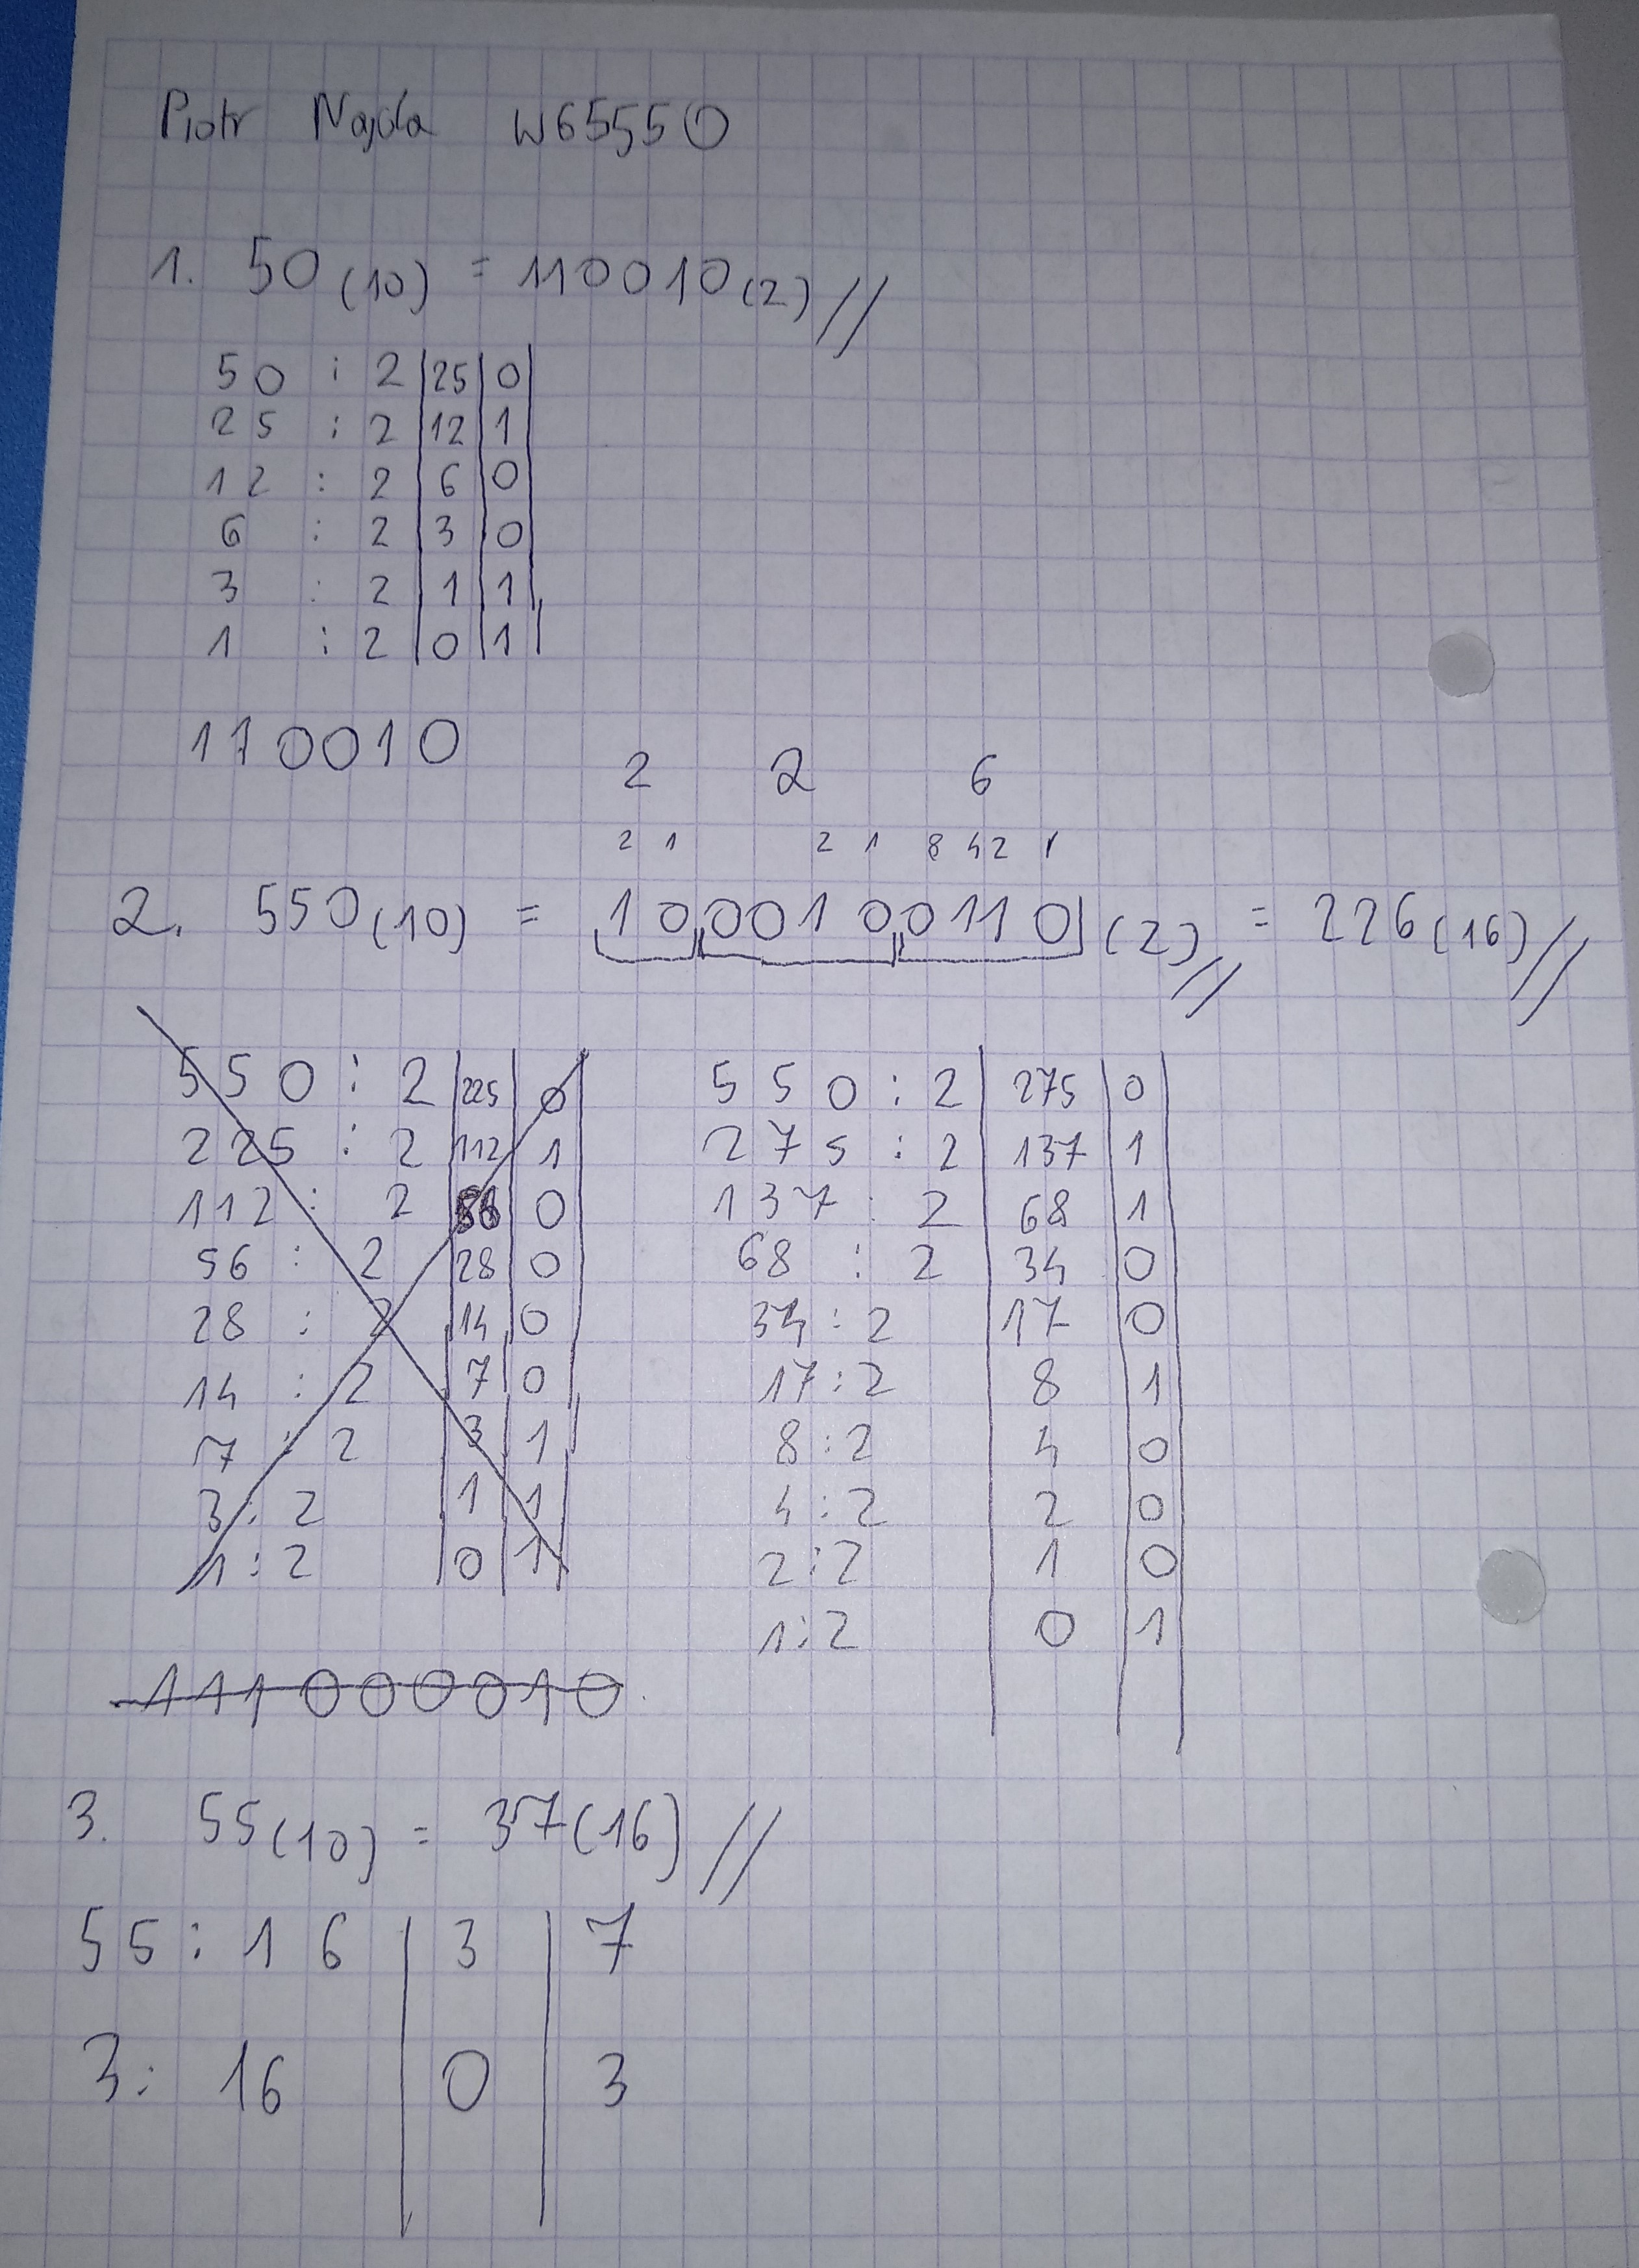
\includegraphics[width=0.65\textwidth]{IMG_20211026_084539.jpg}
\caption{\label{fig:zad1do3}Zadania 1-3}
\end{figure}

\begin{figure}[t]
\centering
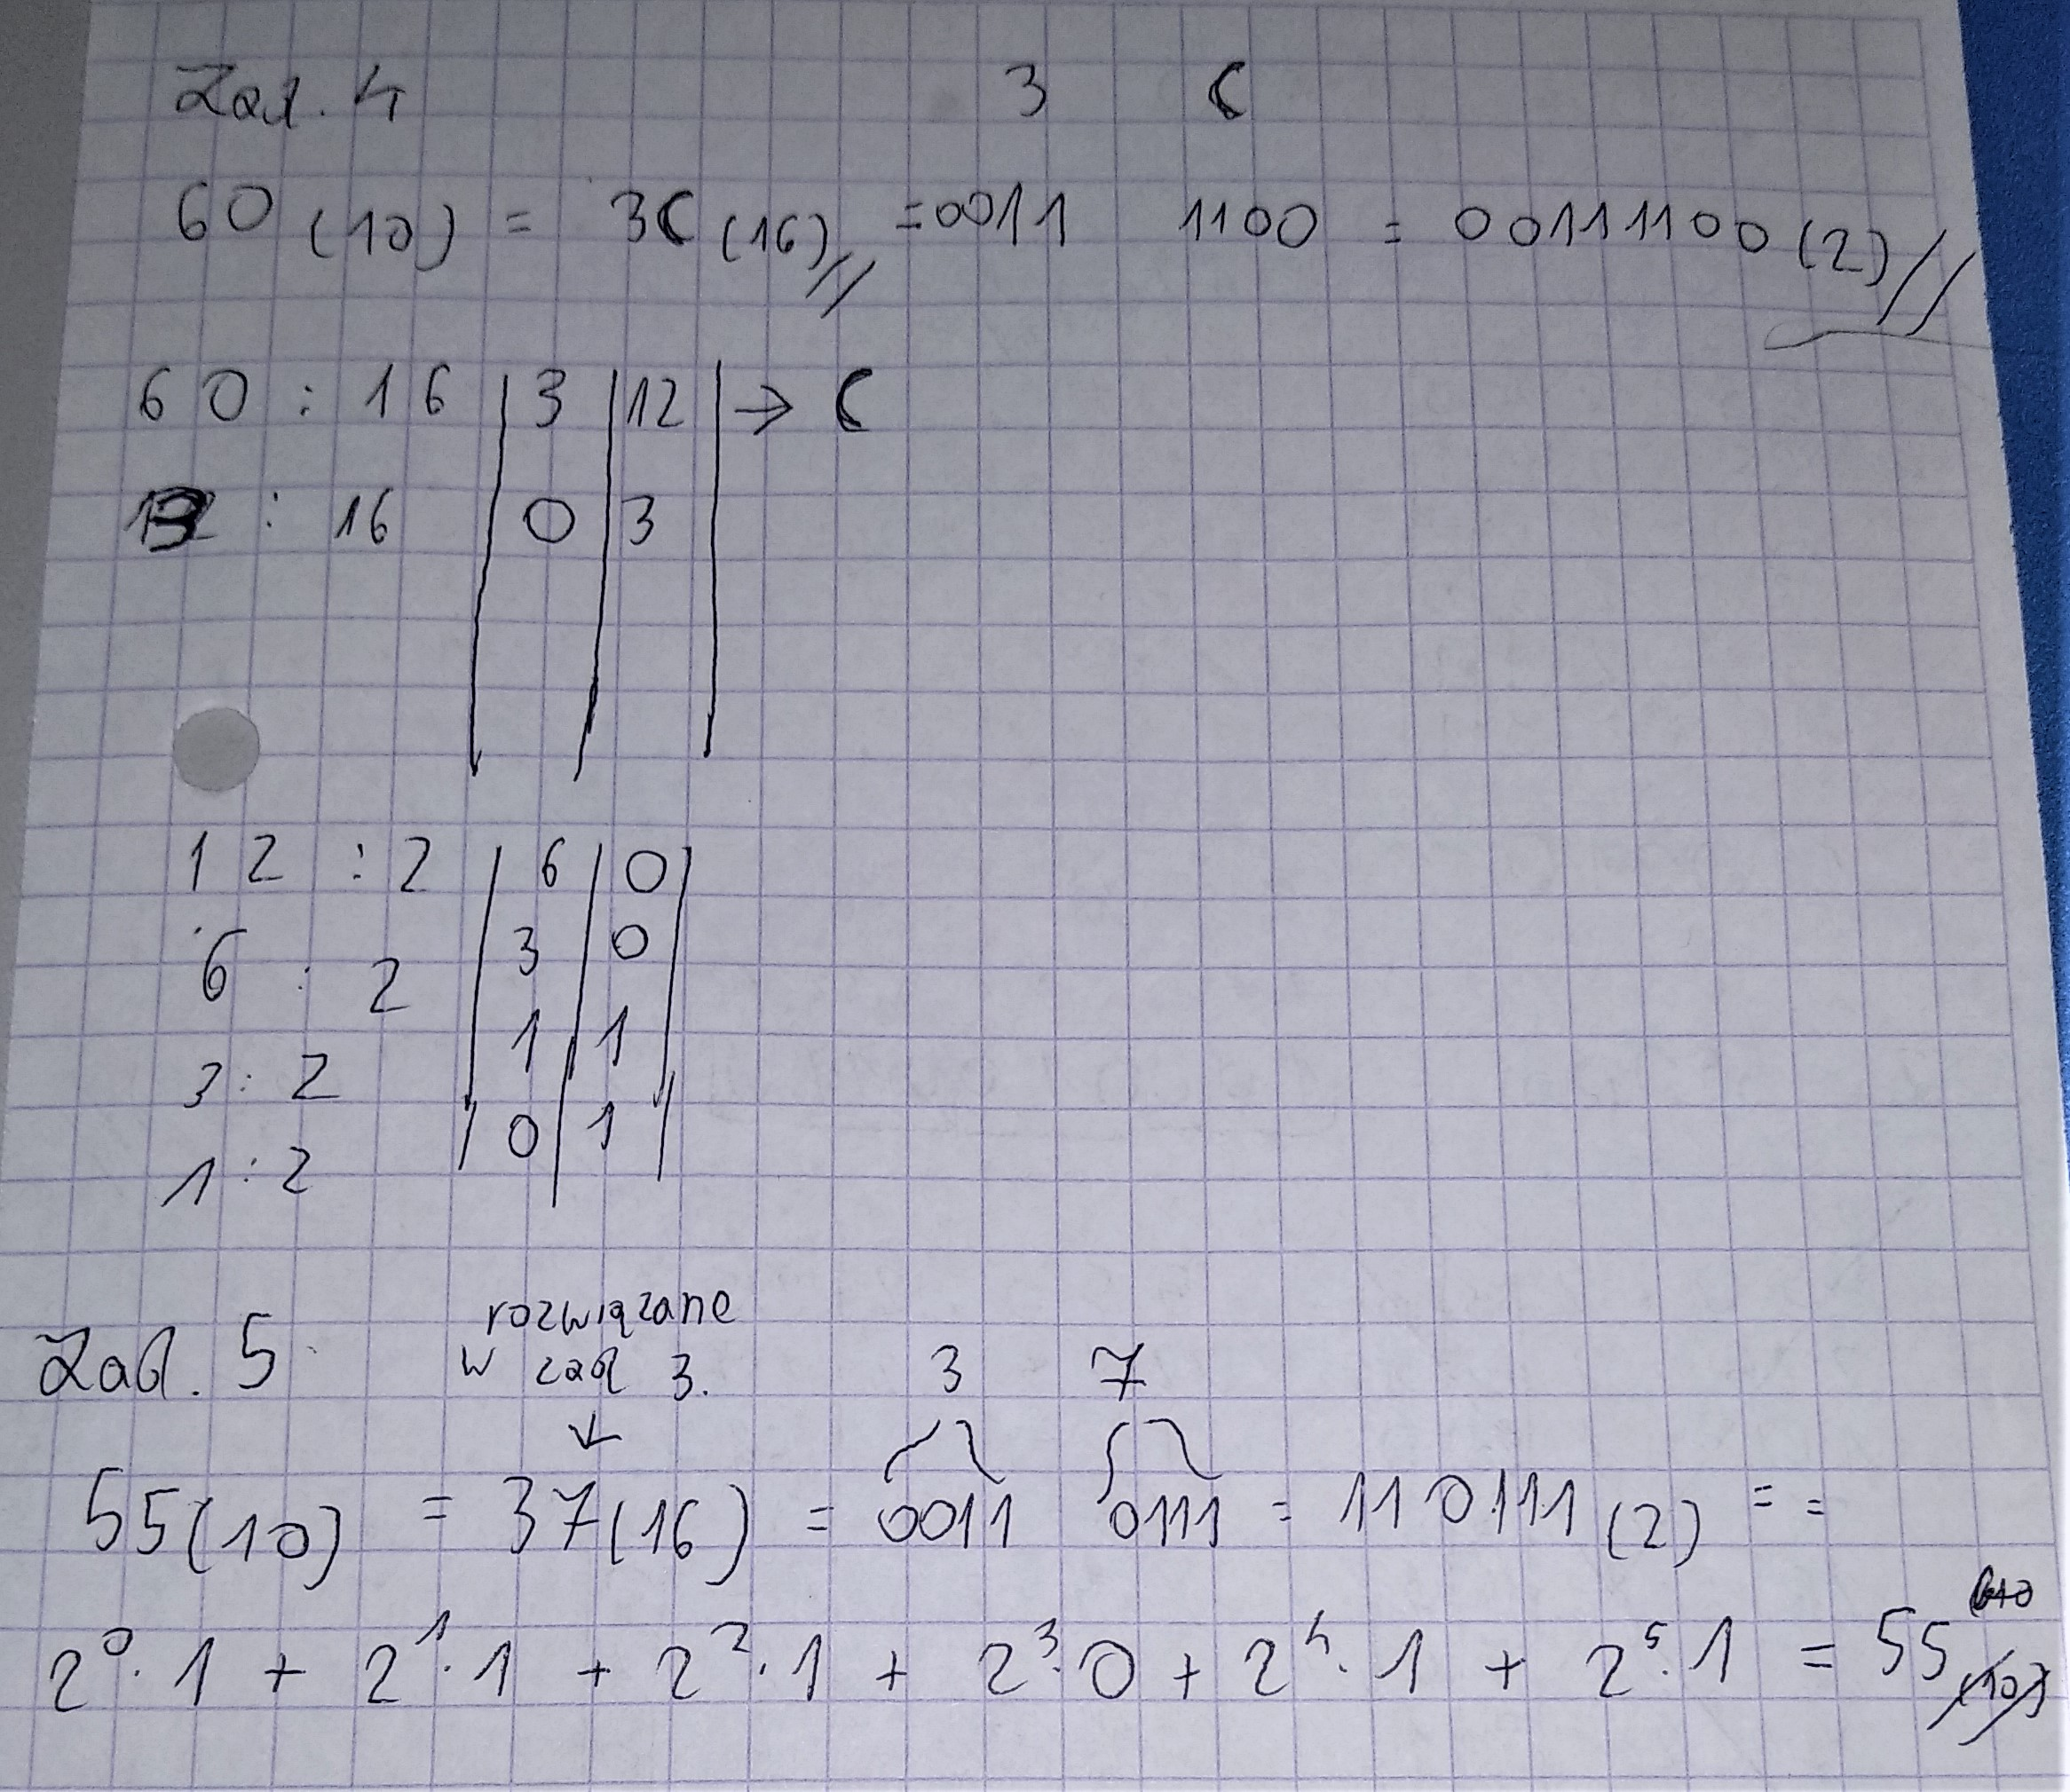
\includegraphics[width=0.99\textwidth]{IMG_20211026_084546.jpg}
\caption{\label{fig:zad4do5}Zadania 4-5}
\end{figure}

\section{Zadania dodatkowe}

\subsection{Punkty a - b}

Wykonałem zadanie w Excelu z użyciem makr, które służą do poprawnego działania tej części zadania. 

\subsection{Algorytm hornera}

\begin{itemize}
    \item Brak cyfry proszę wpisywać jako puste pole, nie jako 0 
    \item Wynik podkreślany jest na żółto
\end{itemize}

\end{document}